\documentclass[xcolor=x11names,compress,professionalfonts]{beamer}

%% General packages %%%%%%%%%%%%%%%%%%%%%%%%%%%%%%%%%%
\usepackage[utf8]{inputenc}
\usepackage{graphicx}
\usepackage{tikz}
\tikzset{% change default arrow tips
    >=latex
}
\usepackage{ifthen}

\usepackage{amsmath}
\usepackage{nicefrac}

\usepackage{color}

%%%%%%%%%%%%%%%%%%%%%%%%%%%%%%%%%%%%%%%%%%%%%%%%%%%%%%

\makeatletter
\setbeamertemplate{footline}
{
    \leavevmode%
    \hbox{%
        \begin{beamercolorbox}[wd=.333333\paperwidth,ht=2.25ex,dp=1ex,center]{author in head/foot}%
            \usebeamerfont{author in head/foot}\insertshortauthor
        \end{beamercolorbox}%
                \begin{beamercolorbox}[wd=.333333\paperwidth,ht=2.25ex,dp=1ex,center]{title in head/foot}%
            \usebeamerfont{title in head/foot}\insertshorttitle
        \end{beamercolorbox}%
        \begin{beamercolorbox}[wd=.333333\paperwidth,ht=2.25ex,dp=1ex,right]{date in head/foot}%
            \usebeamerfont{date in head/foot}\insertshortdate{}\hspace*{2em}
            \insertframenumber{} / \inserttotalframenumber\hspace*{2ex} 
        \end{beamercolorbox}}%
        \vskip0pt%
    }
    \makeatother


%% Beamer Layout %%%%%%%%%%%%%%%%%%%%%%%%%%%%%%%%%%
\useoutertheme[subsection=false,shadow]{miniframes}
\useinnertheme{rectangles}

\setbeamertemplate{navigation symbols}{}%remove navigation symbols

\author{Nicolas Macé}

\newcommand{\btVFill}{\vskip0pt plus 1filll}%place an element at the bottom of the page

\usepackage{libertine}
\usepackage[T1]{fontenc}

\setbeamerfont{title like}{shape=\scshape}
\setbeamerfont{frametitle}{shape=\scshape}

\setbeamercolor*{lower separation line head}{bg=DeepSkyBlue4} 
\setbeamercolor*{normal text}{fg=black,bg=white} 
\setbeamercolor*{alerted text}{fg=red} 
\setbeamercolor*{example text}{fg=black} 
\setbeamercolor*{structure}{fg=black} 
 
\setbeamercolor*{palette tertiary}{fg=black,bg=black!10} 
\setbeamercolor*{palette quaternary}{fg=black,bg=black!10} 

\renewcommand{\(}{\begin{columns}}
\renewcommand{\)}{\end{columns}}
\newcommand{\<}[1]{\begin{column}{#1}}
\renewcommand{\>}{\end{column}}

\definecolor{BostonBlue}{HTML}{00688B}
\definecolor{Complementary}{HTML}{8B2300}

\renewcommand{\ss}[1]{\scriptsize{\text{#1}}}
%%%%%%%%%%%%%%%%%%%%%%%%%%%%%%%%%%%%%%%%%%%%%%%%%%

\usepackage{braket}
% compile child documents using this preamble
\usepackage{subfiles}

%%%My Math

\newcommand{\pd}[2]{\frac{\displaystyle \partial #1}{\displaystyle\partial #2}} % for partial derivatives
\renewcommand{\d}[1]{\mathrm{d}#1}

\begin{document}

\begin{frame}
\frametitle{Examples of wavefunctions on quasiperiodic tilings}
\tableofcontents[hideallsubsections]
\end{frame}

\section{A baby example (Fibonacci tiling)}
%Each section needs a subsection for the small points on top to show up
\subsection{Dummy}
\begin{frame}{Construction of the model}

		The geometrical model:
		
		{\centering
		\includegraphics[scale=0.8]{img/cut_and_project_Fibonacci.pdf}
		
		}
		
		The corresponding chain of atoms:
		
		{\centering
		\includegraphics[scale=1.2]{img/chain_for_inset.pdf}
		
		}
\[
	 t_{m-1,m} \psi_{m-1} + t_{m,m+1}\psi_{m+1} = E \psi_{m}
\]
\[
	t_{=\joinrel=} = 1,~t_{-\joinrel-} = \rho,~\rho<1
\]

\end{frame}

\begin{frame}{Spectrum}

{\centering
\includegraphics[scale=.5]{img/ldos.pdf}

}

$E=0$ is in the spectrum. We will focus on the associated state.

\end{frame}

\begin{frame}{The height function}

{\centering
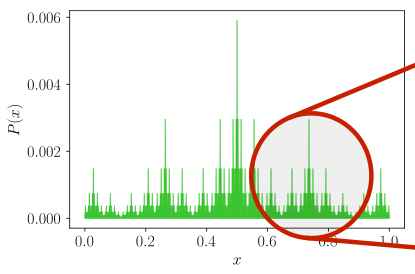
\includegraphics[scale=.5]{img/heights.pdf}

}

\begin{itemize}
	\item The arrow function is quasiperiodic (?).
	\item Its integral, the height function, has logarithmic growth.
\end{itemize}
\end{frame}

\begin{frame}{The $E=0$ wavefunction}

{\centering
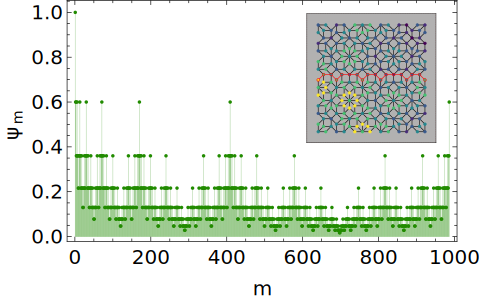
\includegraphics[scale=.8]{img/wavefunction.pdf}

}

\end{frame}

\begin{frame}{Recap}

\begin{itemize}
	\item Wavefunction construction involves a geometrical quasiperiodic function,
	\item Its integral, the height function, has logarithmic growth,
	\item This implies power law behavior of the wavefunction,
	\item The wavefunction is somewhat inbetween localized and extended.
\end{itemize}
$\rightarrow$ We will find again all theses features in the Ammann-Beenker case.
\end{frame}

\section{A grown-up example (Ammann-Beenker tiling)}
%Each section needs a subsection for the small points on top to show up
\subsection{Dummy}
\begin{frame}{Construction of the model}

\begin{columns}

\begin{column}{5cm}
{\centering
\includegraphics[scale=.1]{img/ammann-beenker.png}

}
\end{column}

\begin{column}{5cm}
\[
	-\sum_{n \in V(m)} \psi_n = E \psi_m
\]

No parameters: the quasiperiodic features are encoded in the adjacency of the vertices.
\end{column}
\end{columns}

\end{frame}

\begin{frame}{The height function}

\begin{columns}

\begin{column}{8cm}
{\centering
\includegraphics[scale=.5]{img/heights_ammann.png}

}
\end{column}

\begin{column}{4cm}

\begin{itemize}
	\item The arrow function is quasiperiodic.
	\item Its integral, the height function, has logarithmic growth.
\end{itemize}
\end{column}
\end{columns}

\end{frame}

\begin{frame}{The groundstate wavefunction}

{\centering
\includegraphics[scale=.55]{img/wf_num_infl_6.png}

}

\end{frame}

\begin{frame}{Localization degree of the wavefunction}

\[
D(\psi) = \lim_{R \to \infty} \frac{\log \text{PR}(\psi,R)}{\log \text{Vol}(R)}
\]

\[
D(\psi_{GS}) = \log\left( \frac{\omega(\beta_{GS}^2)^2}{\omega(\beta_{GS}^4)}\right)/\log \omega(1)
\]
with 
\[ 
\omega(z) = \frac{4 +9 z + 4 z^2+2 \sqrt{2} \sqrt{2 z^4+9 z^3+14 z^2+9 z+2}}{z}
\]

{\centering
\includegraphics[scale=.4]{img/coeffPR.pdf}

}

\end{frame}

\begin{frame}{Tuning the localization degree}

\[
-t \sum_{n \in V(m)} \psi_n + (1-t)z_m \psi_m = E \psi_m
\]

\begin{columns}
\begin{column}{5cm}
\includegraphics[scale=.4]{img/coeffPR.pdf}
\end{column}

\begin{column}{5cm}
\includegraphics[scale=.4]{img/beta_t.pdf}
\end{column}

\end{columns}

\end{frame}

\begin{frame}{Recap}
\begin{itemize}
	\item Wavefunction construction involves a geometrical quasiperiodic function,
	\item Its integral, the height function, has logarithmic growth,
	\item This implies power law behavior of the wavefunction (plus some local variations),
	\item The wavefunction is somewhat inbetween localized and extended,
	\item The localization degree of the wavefunction can be varied by tuning the model.
\end{itemize}
\end{frame}

\end{document}